\section{Design Requirements}
The goal for the prototype is to define which way to control the 3D virtual environment is the most familiar one for the user and also the most intuitive one. As mentioned in User Experience chapter (\ref{UXStrategy}), familiarity is very related to intuitiveness.

For the project to answer the question of minimizing the knowledge gap through the concept of familiarity, several design requirements need to be established:

\begin{itemize}
\item Uphold one of the two conditions from the knowledge gap (section \ref{KnowledgeGap})\
\item Make UI elements stand out through the use of isolation (section \ref{IsolationEffect})\
\item Make use of gyroscope in terms of reflecting real life movement\
\item Stick to one color scheme\
\item Limit amount of information given to the user\
\end{itemize}

In the following section, these requirements will be covered.

The prototype needed to have two features to navigate in 3D virtual environment - the moving of the character and the camera movement/rotation. The familiarity concept was put into effect as the control schemes for controlling the environment had to be linked with something that the user might be familiar with already. It was chosen to make extremities of the control schemes to establish familiarity in distinct ways.

The currently existing sensors in mobiles enable the creation of unusual ways of controlling a 3d environment. With the goal in mind of achieving familiarity and intuitivity through the non-traditional sensors, two different approaches to familiarity were established. The knowledge and familiarity to the currently existing products on the market (State of the Art, \ref{SOTA}), and the familiarity of movement representative to the one of movement in real life. For both approaches the current and the target knowledge (\ref{KnowledgeGap}), points for the user are expected to be separate. The design needs to be established in a way to help the users get through the knowledge gap intuitively, when they are involved in the designed task. 


\subsection{Control Schemes}
\subsubsection{Gyroscopic Controls}
Establishing the gyroscopic sensor creates a possibility to interact in an unusual, but familiar way. It enables the prototype to be built around what is most familiar to the real life in movement - actual moving around in reality to navigate.

Controlling the camera with an in-built gyroscope in the tablet is familiar with a natural way for a person to look around - by turning the direction user wishes to move. The movement forward and backwards was implemented with on-screen buttons as these were familiar to the target group through the usual daily tasks, since most of the controllers for movement are represented as such (e.g. arrows on the computer keyboard, music player, cell phone).

\subsubsection{Joystick}
In this prototype the user has to navigate using two joysticks - one for movement and one for camera movement/rotation. This should be easy to learn for the users that have experienced using a joystick before, and the target group is expected to have some knowledge as of how to a joystick is supposed to work, because of their popularity in arcade and electronic games, where joysticks are placed on game console’s remotes like Sony Playstation series or Microsoft Xbox. Additionally, even for users with no previous joystick controller experience, that should not be a problem, as the control scheme is supposed to borrow the same concept as moving a computer mouse on the screen in the direction that is same as the device movement itself - both use 2d directional movement.

\subsubsection{On-screen Buttons}
The way that should be the most familiar with the users through daily use - only buttons as the way to move both camera and the character. In this case camera would be moved only with arrow keys located on the screen and same for moving around - arrows indicating movement back and forth. This should be familiar with anyone that has used buttons for navigation of any sorts in virtual environment. 

By implementing familiarity concept to navigation, the problem of minimizing the knowledge gap is tangled so that the user is being trained in a way that seems natural.


\subsection{Immediacy and Simplicity}
To communicate information in a simpler, and faster to perceive manner, the designs will be represented by concepts that are already familiar to the user. This means, that to communicate information to the user, graphical elements will be represented as symbols, that indicate either movement or rotation for buttons, and controls that represent an actual joystick, rather than text. At the same time, this emphasizes the concept of affordance\todo{(need ref from the upcoming usability section)}, as the buttons represent mechanical buttons used in traditional types of controllers, as well as with the joystick controls. As discussed in sections \todo{references}(?, ?, ?), this will further shape the familiarity and intuitivity for the application.

\begin{figure}[H]
\centering
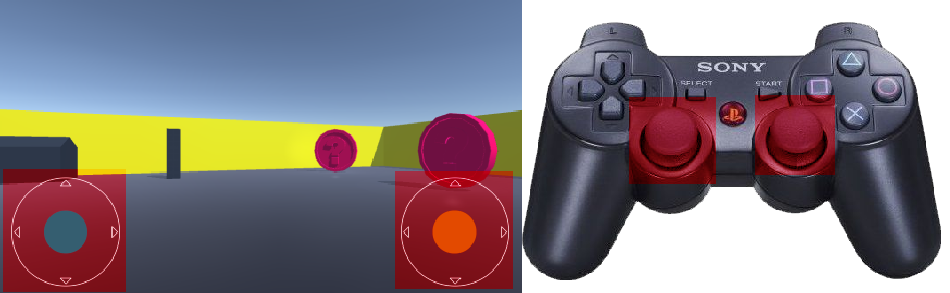
\includegraphics[scale=0.55]{JoystickComparison.png}
\caption{Comparison of initial design sketch of on-screen joystick and the Sony Playstation controller}
\end{figure}

\subsection{Graphical element sizes and placement}
To further emphasize on the user experience\todo{(ref to UX tetraplegia stuff)}, the button size should be set accordingly - to ensure that the users would not have difficulties by unintentionally tapping the wrong section of the controls, individual buttons have to be separated from each other and given the sizes for easy accessibility to reduce the “Fat Finger” problem.
To enable a bigger view of the environment horizontally, the application will be built to primarily be viewed when holding the device in a landscape mode. Since the device is supposed to be held sideways and by both hands, all of the interaction should be done on the sides of the screen, for ease of control access.

To show the difference between movement and rotation controls, they should be given different looks - shape of directional arrows for buttons as well as color indication for both - buttons and joystick controls.

\begin{figure}[H]
\centering
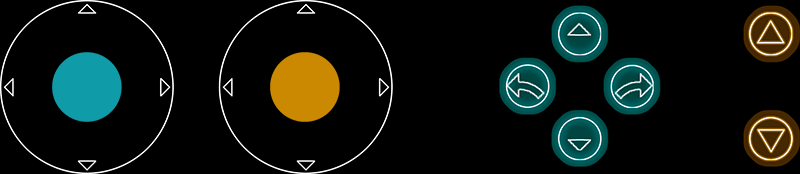
\includegraphics[scale=0.6]{ControllerColors.png}
\caption{Initial sketch. Color differences to distinguish controllers that hold different functions}
\end{figure}

\subsection{Isolation}
To further emphasize on the initial design requirements, the concept of isolation (\ref{IsolationEffect}) should be used when designing the controllers - this should be done by making them stand out from the level content. This is supposed to help the user understand what parts of the application give feedback upon interaction.

\subsection{Conclusion}
These design requirements will help build the necessary prototypes that aim to minimize the knowledge gap using an interface to move in 3d virtual environment on a mobile platform.
